% Document/LinearAlgebra/VectorSpaces/Foundations/Definition.tex
% Section: Vector Spaces - Definition and Basic Properties

\newpage
\section{Vector Spaces}

\begin{remark}[Categorical Perspective]
    Linear algebra studies the category $K$-\textbf{Vect}, where the objects are $K$-vector spaces
    and the morphisms are $K$-linear transformations. This categorical perspective unifies the
    treatment and motivates many constructions we will encounter.
\end{remark}

\begin{definition}[Vector Space]\label{def:vector-space}
    Let $K$ be a field. A \textbf{$K$-vector space} (or \textbf{vector space over $K$}) is a set $V$
    equipped with two operations:
    \begin{itemize}
        \item \textbf{Vector addition}: $+: V \times V \to V$
        \item \textbf{Scalar multiplication}: $\cdot: K \times V \to V$
    \end{itemize}
    satisfying the following axioms for all $u, v, w \in V$ and $a, b \in K$:

    \textbf{Abelian group axioms} (for addition):
    \begin{enumerate}
        \item \textbf{Associativity}: $(u + v) + w = u + (v + w)$
        \item \textbf{Commutativity}: $u + v = v + u$
        \item \textbf{Identity}: $\Exists :{0 \in V}{\Forall :{v \in V}{v + 0 = v}}$
        \item \textbf{Inverses}: $\Forall :{v \in V}{\Exists :{(-v) \in V}{v + (-v) = 0}}$
    \end{enumerate}

    \textbf{Ring action axioms} (for scalar multiplication):
    \begin{enumerate}[resume]
        \item \textbf{Compatibility}: $a(bv) = (ab)v$
        \item \textbf{Identity}: $1_K \cdot v = v$
        \item \textbf{Distributivity over vector addition}: $a(u + v) = au + av$
        \item \textbf{Distributivity over scalar addition}: $(a + b)v = av + bv$
    \end{enumerate}

    Elements of $V$ are called \textbf{vectors}, and elements of $K$ are called \textbf{scalars}.
\end{definition}

\begin{example}[Geometric Vectors in $\bb{R}^2$ and $\bb{R}^3$]\label{ex:geometric-vectors}
    The prototypical example of a vector space is the set of geometric vectors in 2D or 3D space.
    We identify points with their \textbf{position vectors}---arrows from the origin to the point.

    \textbf{Addition} follows the \textbf{tip-to-toe rule}: to add $\vec{u}$ and $\vec{v}$,
    place the tail of $\vec{v}$ at the tip of $\vec{u}$; the sum $\vec{u} + \vec{v}$ is the
    arrow from the origin to the tip of $\vec{v}$. Equivalently, this is the
    \textbf{parallelogram rule}.

    \textbf{Scalar multiplication} scales the vector: $a\vec{v}$ stretches (if $|a| > 1$) or
    shrinks (if $|a| < 1$) the vector, and reverses direction if $a < 0$.

    \begin{center}
    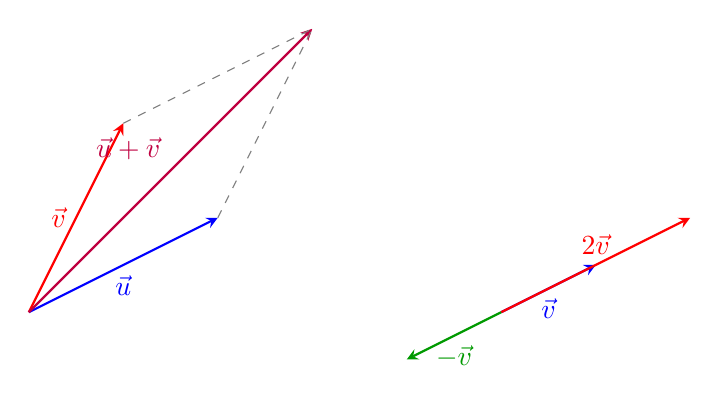
\begin{tikzpicture}[scale=1.2, >=stealth]
        % Parallelogram rule
        \draw[->, thick, blue] (0,0) -- (2,1) node[midway, below] {$\vec{u}$};
        \draw[->, thick, red] (0,0) -- (1,2) node[midway, left] {$\vec{v}$};
        \draw[->, thick, purple] (0,0) -- (3,3) node[midway, above left] {$\vec{u} + \vec{v}$};
        \draw[dashed, gray] (2,1) -- (3,3);
        \draw[dashed, gray] (1,2) -- (3,3);

        % Scalar multiplication
        \begin{scope}[xshift=5cm]
            \draw[->, thick, blue] (0,0) -- (1,0.5) node[midway, below] {$\vec{v}$};
            \draw[->, thick, red] (0,0) -- (2,1) node[midway, above] {$2\vec{v}$};
            \draw[->, thick, green!60!black] (0,0) -- (-1,-0.5) node[midway, below] {$-\vec{v}$};
        \end{scope}
    \end{tikzpicture}
    \end{center}
\end{example}

\begin{example}[Coordinate Spaces $K^n$]\label{ex:coordinate-space}
    For any field $K$ and positive integer $n$, the set
    \[
        K^n = \Set{(x_0, \ldots, x_{n-1}) \mid x_i \in K}
    \]
    forms a $K$-vector space with pointwise operations:
    \begin{align*}
        (x_0, \ldots, x_{n-1}) + (y_0, \ldots, y_{n-1}) &= (x_0 + y_0, \ldots, x_{n-1} + y_{n-1}) \\
        a \cdot (x_0, \ldots, x_{n-1}) &= (ax_0, \ldots, ax_{n-1})
    \end{align*}

    More formally, $K^n = K^{\{0, 1, \ldots, n-1\}}$---the set of functions from the ordinal $n = \{0, 1, \ldots, n-1\}$ to $K$.
    We identify the $n$-tuple $(x_0, \ldots, x_{n-1})$ with the function $i \mapsto x_i$.
\end{example}

\begin{remark}[Geometric Interpretation of $K^n$]\label{rem:geometric-K^n}
    For $n = 1, 2, 3$ over $K = \bb{R}$, we identify points in $\bb{R}^n$ with \textbf{position vectors}:
    arrows from the origin $0$ to the point. This identification is bijective:
    \[
        (x_0, \ldots, x_{n-1}) \longleftrightarrow \text{arrow from } 0 \text{ to } (x_0, \ldots, x_{n-1})
    \]
    Under this identification, the vector space operations on $\bb{R}^n$ correspond exactly to
    the geometric operations on arrows described in Example~\ref{ex:geometric-vectors}.

    \textbf{Why addition matches the parallelogram rule.}
    Let $e_0 = (1, 0)$ and $e_1 = (0, 1)$ be the standard basis vectors.
    Any $u = (u_0, u_1)$ decomposes as $u = u_0 e_0 + u_1 e_1$,
    and similarly $v = v_0 e_0 + v_1 e_1$. Then by the vector space axioms:
    \[
        u + v = (u_0 e_0 + u_1 e_1) + (v_0 e_0 + v_1 e_1)
        = (u_0 + v_0) e_0 + (u_1 + v_1) e_1
    \]
    which corresponds to the point $(u_0 + v_0, \; u_1 + v_1)$.
    Geometrically, this is the fourth vertex of the parallelogram
    formed by $0$, $u$, and $v$: translating the arrow $v$ so that its tail
    is at the tip of $u$ places its tip at $(u_0 + v_0, \; u_1 + v_1)$.

    \begin{center}
    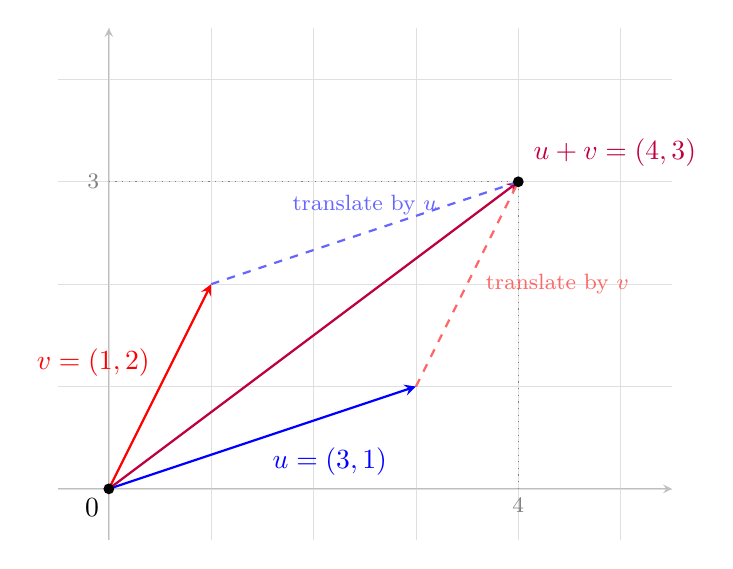
\begin{tikzpicture}[scale=1.3, >=stealth]
        % Grid for coordinates
        \draw[gray!25, very thin] (-0.5,-0.5) grid (5.5,4.5);

        % Axes
        \draw[gray!50, ->] (-0.5,0) -- (5.5,0);
        \draw[gray!50, ->] (0,-0.5) -- (0,4.5);

        % Vectors
        \draw[->, thick, blue] (0,0) -- (3,1) node[midway, below right] {$u = (3,1)$};
        \draw[->, thick, red] (0,0) -- (1,2) node[midway, above left] {$v = (1,2)$};
        \draw[->, thick, purple] (0,0) -- (4,3);

        % Label at tip
        \node[purple, above right=2pt] at (4,3) {$u + v = (4,3)$};

        % Parallelogram sides
        \draw[dashed, blue!60, thick] (1,2) -- (4,3)
            node[midway, above=3pt] {\footnotesize translate by $u$};
        \draw[dashed, red!60, thick] (3,1) -- (4,3)
            node[midway, right=3pt] {\footnotesize translate by $v$};

        % Coordinate projections for u+v
        \draw[dotted, gray] (4,0) node[below] {\footnotesize $4$} -- (4,3);
        \draw[dotted, gray] (0,3) node[left] {\footnotesize $3$} -- (4,3);

        % Points
        \fill (0,0) circle (1.5pt) node[below left] {$0$};
        \fill (4,3) circle (1.5pt);
    \end{tikzpicture}
    \end{center}

    \textbf{Why scalar multiplication matches scaling.}
    For $\alpha \in \bb{R}$ and $u = u_0 e_0 + u_1 e_1$, the scalar multiplication axioms give:
    \[
        \alpha \cdot u = \alpha (u_0 e_0 + u_1 e_1)
        = (\alpha u_0) e_0 + (\alpha u_1) e_1
    \]
    which corresponds to the point $(\alpha u_0, \; \alpha u_1)$.
    Geometrically, this is the point at fraction $\alpha$ along the ray from $0$
    through $u$: it stretches the arrow by $|\alpha|$ and reverses direction if $\alpha < 0$.
    The parametric line $t \mapsto t \cdot u = (t u_0, \; t u_1)$ confirms this.

    \begin{center}
    \begin{tikzpicture}[>=stealth]
        % --- Stretching: alpha = 2 ---
        \begin{scope}[xshift=0cm]
            \draw[gray!25, very thin] (-0.5, -0.5) grid (4.5, 3.5);
            \draw[gray!50, ->] (-0.5,0) -- (4.5,0);
            \draw[gray!50, ->] (0,-0.5) -- (0,3.5);

            \draw[->, thick, blue] (0,0) -- (1.5,1)
                node[midway, below right=-1pt] {\footnotesize $u$};
            \draw[->, thick, purple] (0,0) -- (3,2)
                node[midway, above left=-1pt] {\footnotesize $2u$};

            % Dashed extension
            \draw[dashed, gray!50] (1.5,1) -- (3,2);

            \fill (0,0) circle (1.5pt) node[below left] {\footnotesize $0$};
            \node[below] at (2,-0.9) {$\alpha = 2$ (stretch)};
        \end{scope}

        % --- Squishing: alpha = 1/2 ---
        \begin{scope}[xshift=6cm]
            \draw[gray!25, very thin] (-0.5, -0.5) grid (4.5, 3.5);
            \draw[gray!50, ->] (-0.5,0) -- (4.5,0);
            \draw[gray!50, ->] (0,-0.5) -- (0,3.5);

            \draw[->, thick, blue] (0,0) -- (3,2)
                node[near end, above left=-1pt] {\footnotesize $u$};
            \draw[->, very thick, purple] (0,0) -- (1.5,1)
                node[midway, below right=-1pt] {\footnotesize $\tfrac{1}{2}u$};

            \fill (0,0) circle (1.5pt) node[below left] {\footnotesize $0$};
            \node[below] at (2,-0.9) {$\alpha = \tfrac{1}{2}$ (squish)};
        \end{scope}

        % --- Negation: alpha = -1 ---
        \begin{scope}[xshift=12cm]
            \draw[gray!25, very thin] (-2.5, -2.5) grid (2.5, 2.5);
            \draw[gray!50, ->] (-2.5,0) -- (2.5,0);
            \draw[gray!50, ->] (0,-2.5) -- (0,2.5);

            \draw[->, thick, blue] (0,0) -- (1.5,1)
                node[midway, above left=-1pt] {\footnotesize $u$};
            \draw[->, thick, purple] (0,0) -- (-1.5,-1)
                node[midway, below right=-1pt] {\footnotesize $-u$};

            % Dashed line through both
            \draw[dashed, gray!50] (-2,-1.33) -- (2,1.33);

            \fill (0,0) circle (1.5pt) node[above left] {\footnotesize $0$};
            \node[below] at (0,-2.9) {$\alpha = -1$ (negate)};
        \end{scope}
    \end{tikzpicture}
    \end{center}

    This geometric intuition guides much of linear algebra, even in higher dimensions and over
    abstract fields where visualization is not possible.
\end{remark}

\begin{example}[Function Spaces $K^I$]\label{ex:function-space}
    For any set $I$, the set of all functions $f: I \to K$ forms a $K$-vector space $K^I$ with
    pointwise operations:
    \begin{align*}
        (f + g)(i) &= f(i) + g(i) \\
        (af)(i) &= a \cdot f(i)
    \end{align*}

    For each $i \in I$, define the \textbf{indicator function} $e_i: I \to K$ by
    \[
        e_i(j) = \delta_{ij} =
        \begin{cases}
            1_K & \text{if } j = i \\
            0_K & \text{if } j \neq i
        \end{cases}
    \]
    These indicator functions will play a central role once we introduce bases.
\end{example}

\begin{example}[Functions with Finite Support $K^{(I)}$]\label{ex:finite-support}
    The set of functions with \textbf{finite support}
    \[
        K^{(I)} = \Set{f \in K^I \mid \Set{i \in I \mid f(i) \neq 0} \text{ is finite}}
    \]
    is a subspace of $K^I$. Every $f \in K^{(I)}$ can be written as a finite sum
    \[
        f = \sum_{i \in \operatorname{supp}(f)} f(i) \cdot e_i
    \]
    where $\operatorname{supp}(f) = \Set{i \in I \mid f(i) \neq 0}$ is the support of $f$.

    Note that $K^{(I)} = K^I$ if and only if $I$ is finite.
\end{example}

\begin{remark}[Column Vector Notation for $K^n$]\label{rem:column-notation}
    For $n \in \bb{N}$, the elements of $K^n = K^{\{0, 1, \ldots, n-1\}}$ are functions from
    $\{0, 1, \ldots, n-1\}$ to $K$, i.e., finite-length sequences. We denote these as
    \textbf{column vectors}:
    \[
        f \longleftrightarrow
        \ColVec{f(0) \\ f(1) \\ \vdots \\ f(n-1)}
    \]
    For instance, the indicator functions in $K^n$ are denoted
    \[
        e_0 = \ColVec{1 \\ 0 \\ \vdots \\ 0}, \quad
        e_1 = \ColVec{0 \\ 1 \\ \vdots \\ 0}, \quad \ldots, \quad
        e_{n-1} = \ColVec{0 \\ 0 \\ \vdots \\ 1}
    \]
    and a general element $(a_0, a_1, \ldots, a_{n-1}) \in K^n$ is written as
    $\ColVec{a_0 \\ a_1 \\ \vdots \\ a_{n-1}}$.
\end{remark}

\begin{example}[Polynomial Spaces]\label{ex:polynomial-space}
    For a field $K$, the polynomial ring $K[X]$ is a $K$-vector space. We define 
    important subspaces based on degree constraints:
    \begin{itemize}
        \item $K[X]_{\leq n} = \Set{p \in K[X] \mid \deg p \leq n}$ (polynomials of degree at most $n$)
        \item $K[X]_{< n} = \Set{p \in K[X] \mid \deg p < n}$ (polynomials of degree less than $n$)
    \end{itemize}
\end{example}

\begin{example}[Matrix Spaces]\label{ex:matrix-space}
    For positive integers $m, n$, the set $\MatSpace{m}{n}[K]$ of $m \times n$ matrices with
    entries in $K$ forms a $K$-vector space with entrywise operations:
    \begin{align*}
        (A + B)_{ij} &= A_{ij} + B_{ij} \\
        (aA)_{ij} &= a \cdot A_{ij}
    \end{align*}
\end{example}

\begin{example}[Field Extensions]\label{ex:field-extension}
    When $L$ is a field extension of $K$ (i.e., $K \subseteq L$ as fields), then $L$ is naturally
    a $K$-vector space with the restriction of multiplication in $L$ as scalar multiplication.
    \begin{itemize}
        \item $\bb{C}$ is a 2-dimensional $\bb{R}$-vector space (basis: $\{1, i\}$)
        \item $\bb{R}$ is an infinite-dimensional $\bb{Q}$-vector space
    \end{itemize}
\end{example}

\begin{proposition}[Basic Properties]\label{prop:vs-basic-properties}
    Let $V$ be a $K$-vector space. The following properties hold for all $v \in V$ and $a \in K$:
    \begin{enumerate}
        \item $0_K \cdot v = 0_V$
        \item $a \cdot 0_V = 0_V$
        \item $(-1_K) \cdot v = -v$
        \item $av = 0_V \implies a = 0_K \LogicOr v = 0_V$
    \end{enumerate}
\end{proposition}

\begin{proof}
    We prove each property:

    \textbf{(1)} We have $0_K \cdot v = (0_K + 0_K) \cdot v = 0_K \cdot v + 0_K \cdot v$.
    Adding $-(0_K \cdot v)$ to both sides yields $0_V = 0_K \cdot v$.

    \textbf{(2)} We have $a \cdot 0_V = a \cdot (0_V + 0_V) = a \cdot 0_V + a \cdot 0_V$.
    Adding $-(a \cdot 0_V)$ to both sides yields $0_V = a \cdot 0_V$.

    \textbf{(3)} We have $v + (-1_K) \cdot v = 1_K \cdot v + (-1_K) \cdot v = (1_K + (-1_K)) \cdot v = 0_K \cdot v = 0_V$.
    By uniqueness of additive inverses, $(-1_K) \cdot v = -v$.

    \textbf{(4)} Suppose $av = 0_V$ and $a \neq 0_K$. Since $K$ is a field, $a^{-1}$ exists.
    Then $v = 1_K \cdot v = (a^{-1}a) \cdot v = a^{-1}(av) = a^{-1} \cdot 0_V = 0_V$.
\end{proof}

\begin{proposition}[Cancellation Laws]\label{prop:cancellation}
    Let $V$ be a $K$-vector space. Then:
    \begin{enumerate}
        \item If $av = bv$ and $v \neq 0_V$, then $a = b$.
        \item If $av = aw$ and $a \neq 0_K$, then $v = w$.
    \end{enumerate}
\end{proposition}

\begin{proof}
    \textbf{(1)} From $av = bv$ we get $av - bv = 0_V$, hence $(a - b)v = 0_V$.
    Since $v \neq 0_V$, by Proposition~\ref{prop:vs-basic-properties}(4), we have $a - b = 0_K$,
    so $a = b$.

    \textbf{(2)} From $av = aw$ we get $a(v - w) = 0_V$.
    Since $a \neq 0_K$, by Proposition~\ref{prop:vs-basic-properties}(4), we have $v - w = 0_V$,
    so $v = w$.
\end{proof}

\begin{remark}[Notation Abuse]
    We use $0$ to denote both the zero scalar $0_K$ and the zero vector $0_V$.
    Context will always make the intended meaning clear.
\end{remark}
